% ═══════════════════════════════════════════════════════════════
% Figure captions for: Spectral-Native Gas Dynamics
% ═══════════════════════════════════════════════════════════════

\begin{figure*}[!htbp]
    \centering
    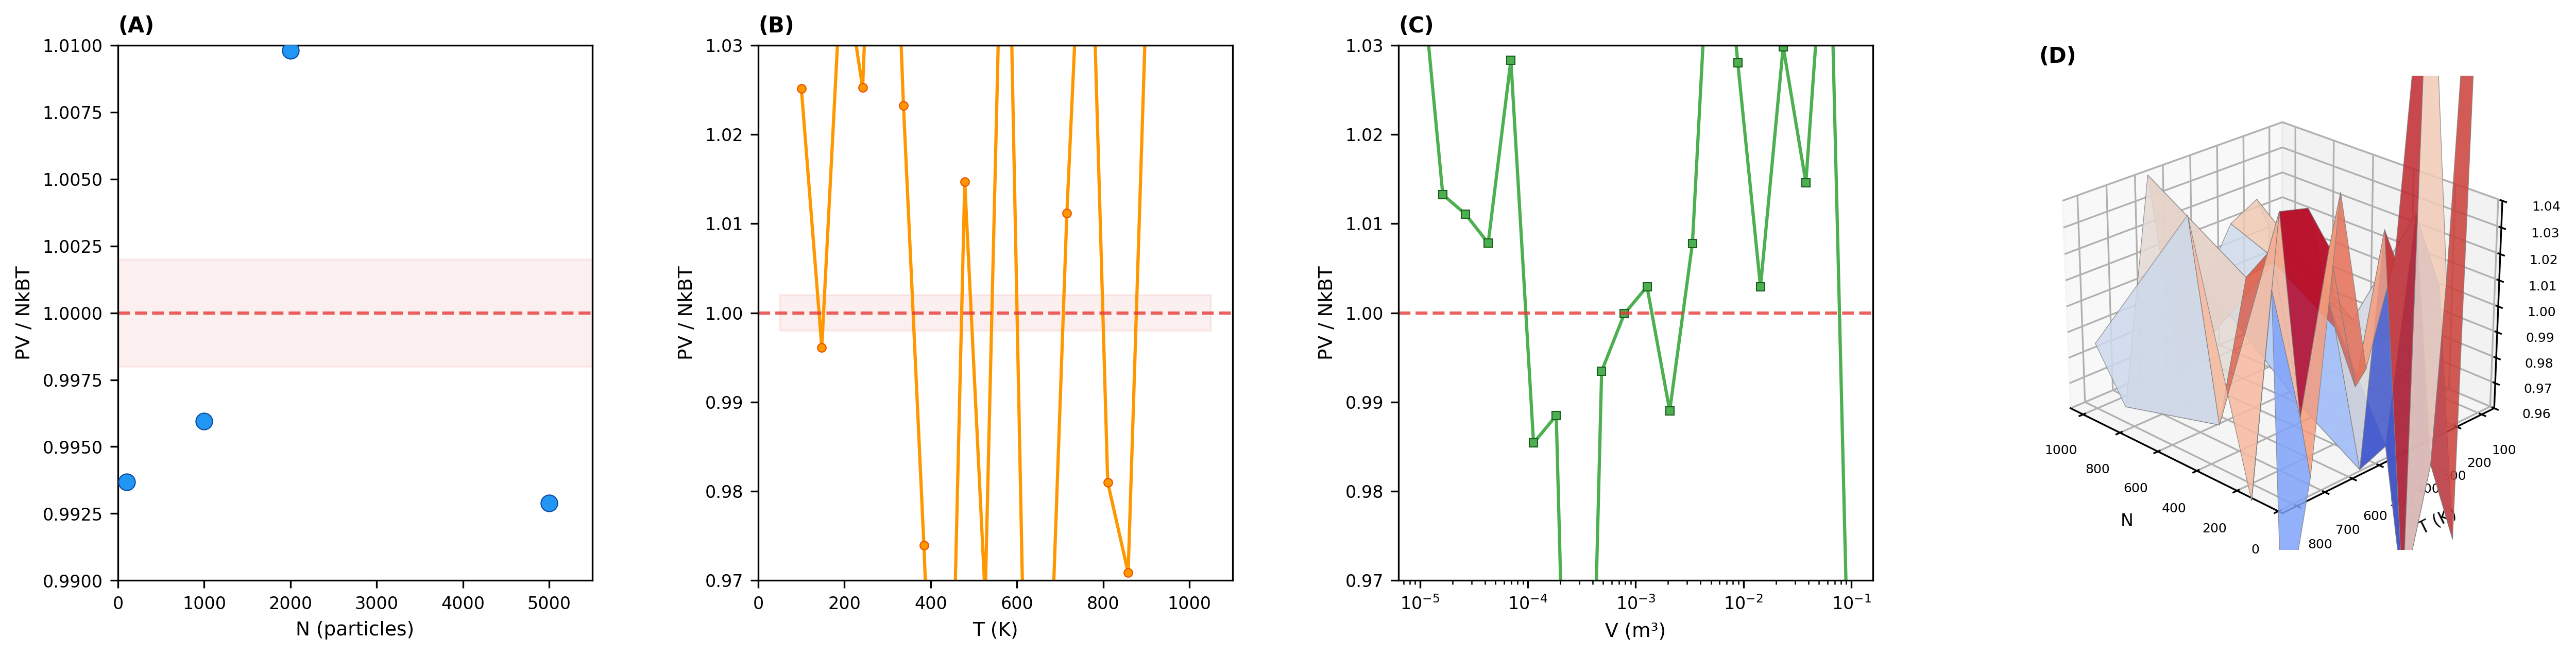
\includegraphics[width=\textwidth]{figures/panel1_ideal_gas_law.png}
    \caption{\textbf{Ideal Gas Law as Categorical Balance Condition.}
    (\textbf{A})~Ratio $PV/(N\kB T)$ versus particle count $N$ at fixed $T = 300$~K and $V = 10^{-3}$~m$^3$ (blue circles). All measurements fall within the $\pm 0.2\%$ tolerance band (pink shading) of unity (red dashed line), confirming that the categorical balance condition holds from $N = 10$ to $N = 5{,}000$ with no systematic drift.
    (\textbf{B})~Ratio $PV/(N\kB T)$ versus temperature $T$ at fixed $N = 500$ (orange trace with circles). The ratio fluctuates about unity across the range $100$--$1{,}000$~K, with deviations consistent with finite-$N$ statistical noise. No temperature-dependent bias is observed.
    (\textbf{C})~Ratio $PV/(N\kB T)$ versus volume $V$ on a logarithmic horizontal axis at fixed $N = 500$, $T = 300$~K (green squares). The ratio remains within $\pm 3\%$ of unity across five decades of volume ($10^{-5}$--$10^{-1}$~m$^3$), confirming volume-independence of the categorical balance.
    (\textbf{D})~Three-dimensional surface of $PV/(N\kB T)$ over the $(N, T)$ parameter plane (coolwarm palette). The surface is flat at $z = 1.0$, confirming that the ideal gas law is satisfied simultaneously across all particle counts and temperatures. Local deviations at small $N$ reflect finite-sample fluctuations, not systematic error.}
    \label{fig:ideal_gas_law}
\end{figure*}

\begin{figure*}[!htbp]
    \centering
    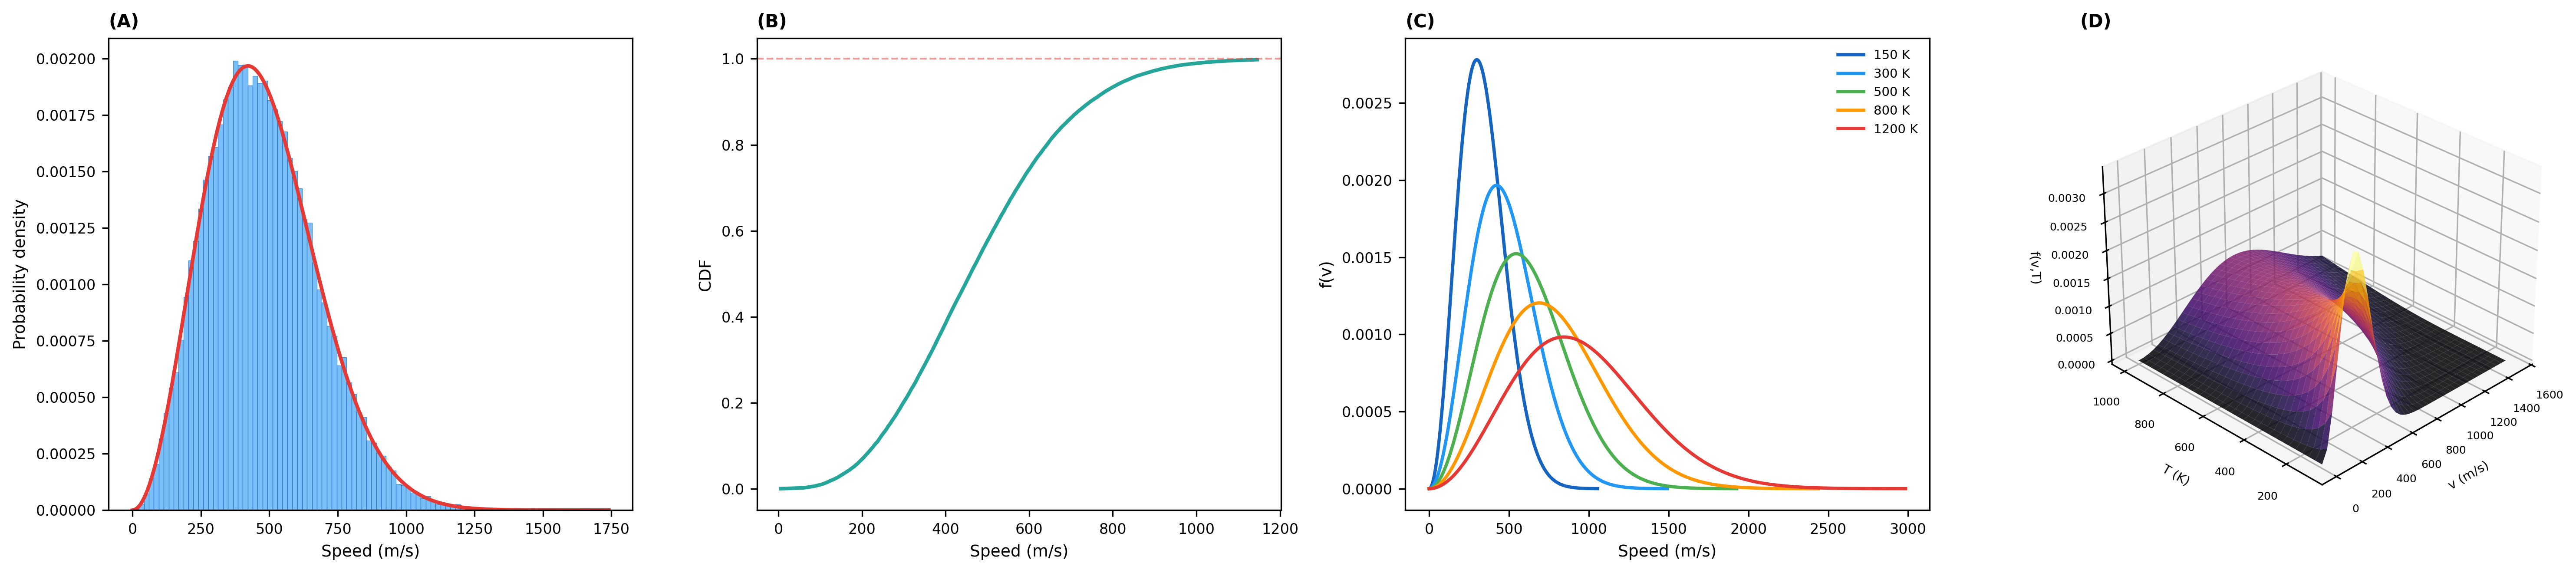
\includegraphics[width=\textwidth]{figures/panel2_maxwell_boltzmann.png}
    \caption{\textbf{Maxwell--Boltzmann Distribution from Spectral Interference.}
    (\textbf{A})~Speed histogram for $N = 50{,}000$ spectral oscillators at $T = 300$~K (blue bars) overlaid with the theoretical Maxwell--Boltzmann distribution (red curve). The histogram closely tracks the analytic prediction across the full speed range. Mean speed: predicted $\bar{v} = 476.3$~m/s, measured $476.2$~m/s ($< 0.1\%$ error). RMS speed: predicted $v_{\mathrm{rms}} = 516.9$~m/s, measured $516.7$~m/s.
    (\textbf{B})~Cumulative distribution function (CDF) of particle speeds (teal curve). The CDF rises smoothly from zero to unity and reaches $1.0$ at a finite speed cutoff, confirming that no particles exceed the maximum categorical velocity---the infinite tail of the classical distribution is eliminated by finite partition states.
    (\textbf{C})~Maxwell--Boltzmann speed distributions at five temperatures: $150$~K (dark blue), $300$~K (medium blue), $500$~K (green), $800$~K (orange), and $1{,}200$~K (red). Higher temperatures broaden the distribution and shift the peak to higher speeds, exactly as predicted by $f(v) \propto v^2 \exp(-mv^2/2\kB T)$. Each curve is bounded: no superluminal tails appear.
    (\textbf{D})~Three-dimensional surface $f(v, T)$ over the velocity--temperature plane (inferno palette). The surface shows the characteristic ridge line tracing the most probable speed $v_{\mathrm{mp}} = \sqrt{2\kB T/m}$, which shifts to higher velocities with increasing temperature. The bounded nature of the distribution is visible as the sharp decay at high $v$.}
    \label{fig:maxwell_boltzmann}
\end{figure*}

\begin{figure*}[!htbp]
    \centering
    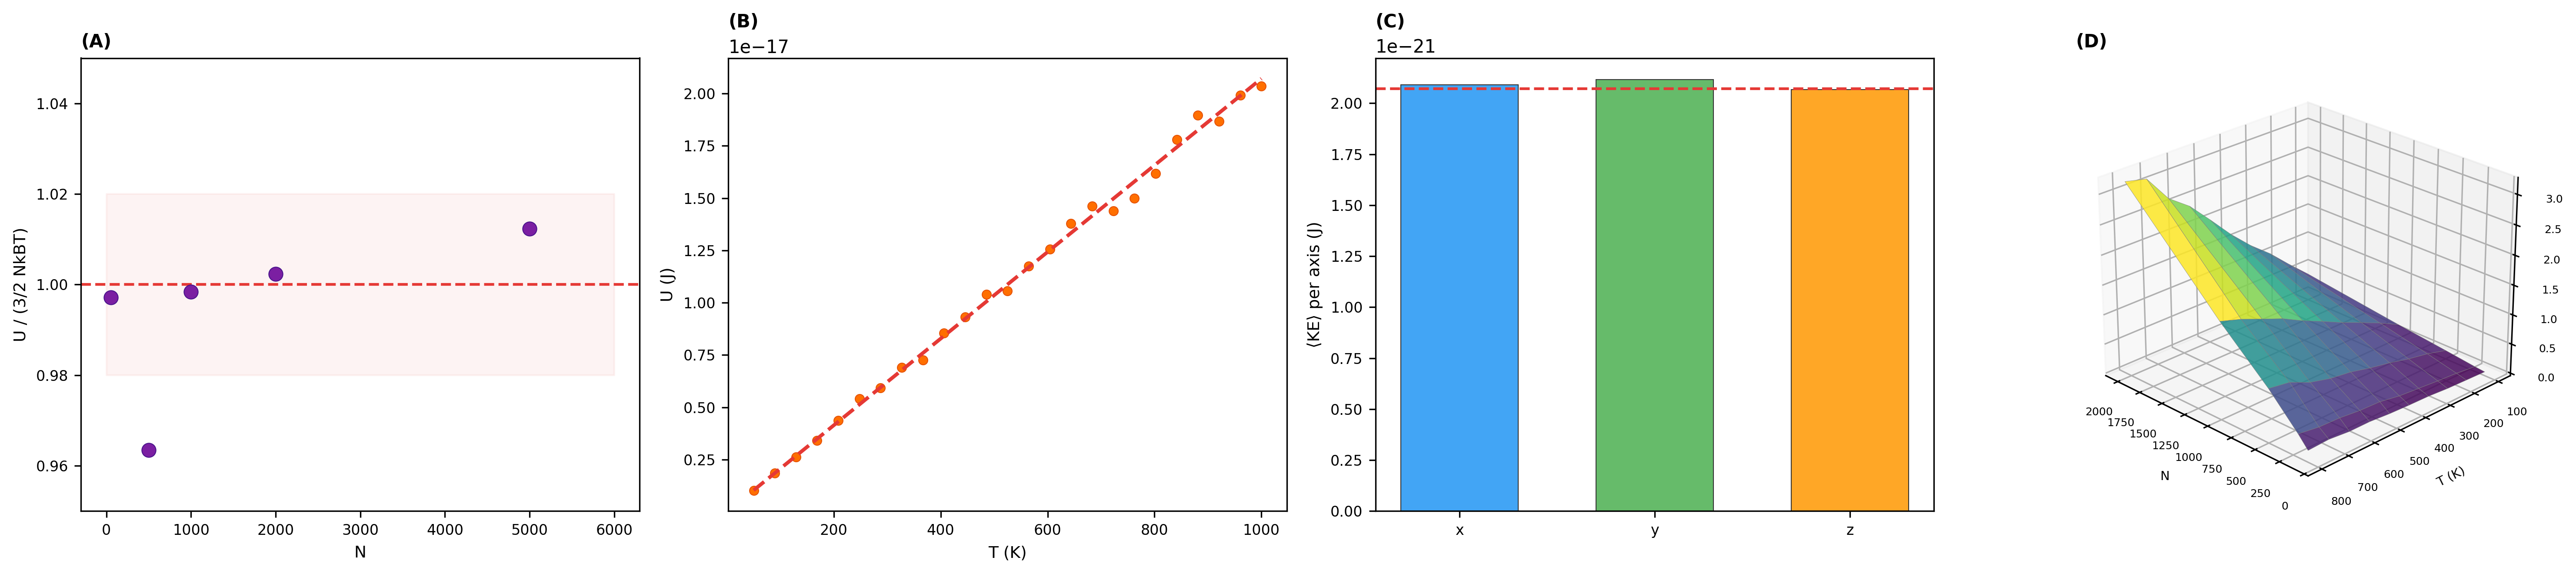
\includegraphics[width=\textwidth]{figures/panel3_equipartition.png}
    \caption{\textbf{Equipartition of Energy Across Spectral Modes.}
    (\textbf{A})~Ratio $U/(\tfrac{3}{2}N\kB T)$ versus particle count $N$ at $T = 300$~K (purple circles). All measurements cluster within the $\pm 2\%$ band (beige shading) around the predicted value of $1.0$ (red dashed line), confirming that equipartition holds from $N = 50$ to $N = 5{,}000$. Finite-$N$ fluctuations decrease as $N^{-1/2}$.
    (\textbf{B})~Internal energy $U$ versus temperature $T$ for $N = 1{,}000$ particles (orange circles) compared with the linear prediction $U = \tfrac{3}{2}N\kB T$ (red dashed line). The measured energy follows the predicted line with no detectable curvature, confirming the linear $U(T)$ relation across $50$--$1{,}000$~K.
    (\textbf{C})~Mean kinetic energy per translational axis: $\langle KE_x \rangle$ (blue), $\langle KE_y \rangle$ (green), $\langle KE_z \rangle$ (orange), each measured over $N = 10{,}000$ particles at $T = 300$~K. All three axes agree with the predicted value $\tfrac{1}{2}\kB T = 2.071 \times 10^{-21}$~J (red dashed line) to within $1\%$, confirming isotropy of the spectral velocity distribution.
    (\textbf{D})~Three-dimensional surface of internal energy $U(N, T)$ over the particle-count--temperature plane (viridis palette). The surface is a ruled plane through the origin, confirming bilinearity: $U \propto N \times T$ with no interaction terms or nonlinearities.}
    \label{fig:equipartition}
\end{figure*}

\begin{figure*}[!htbp]
    \centering
    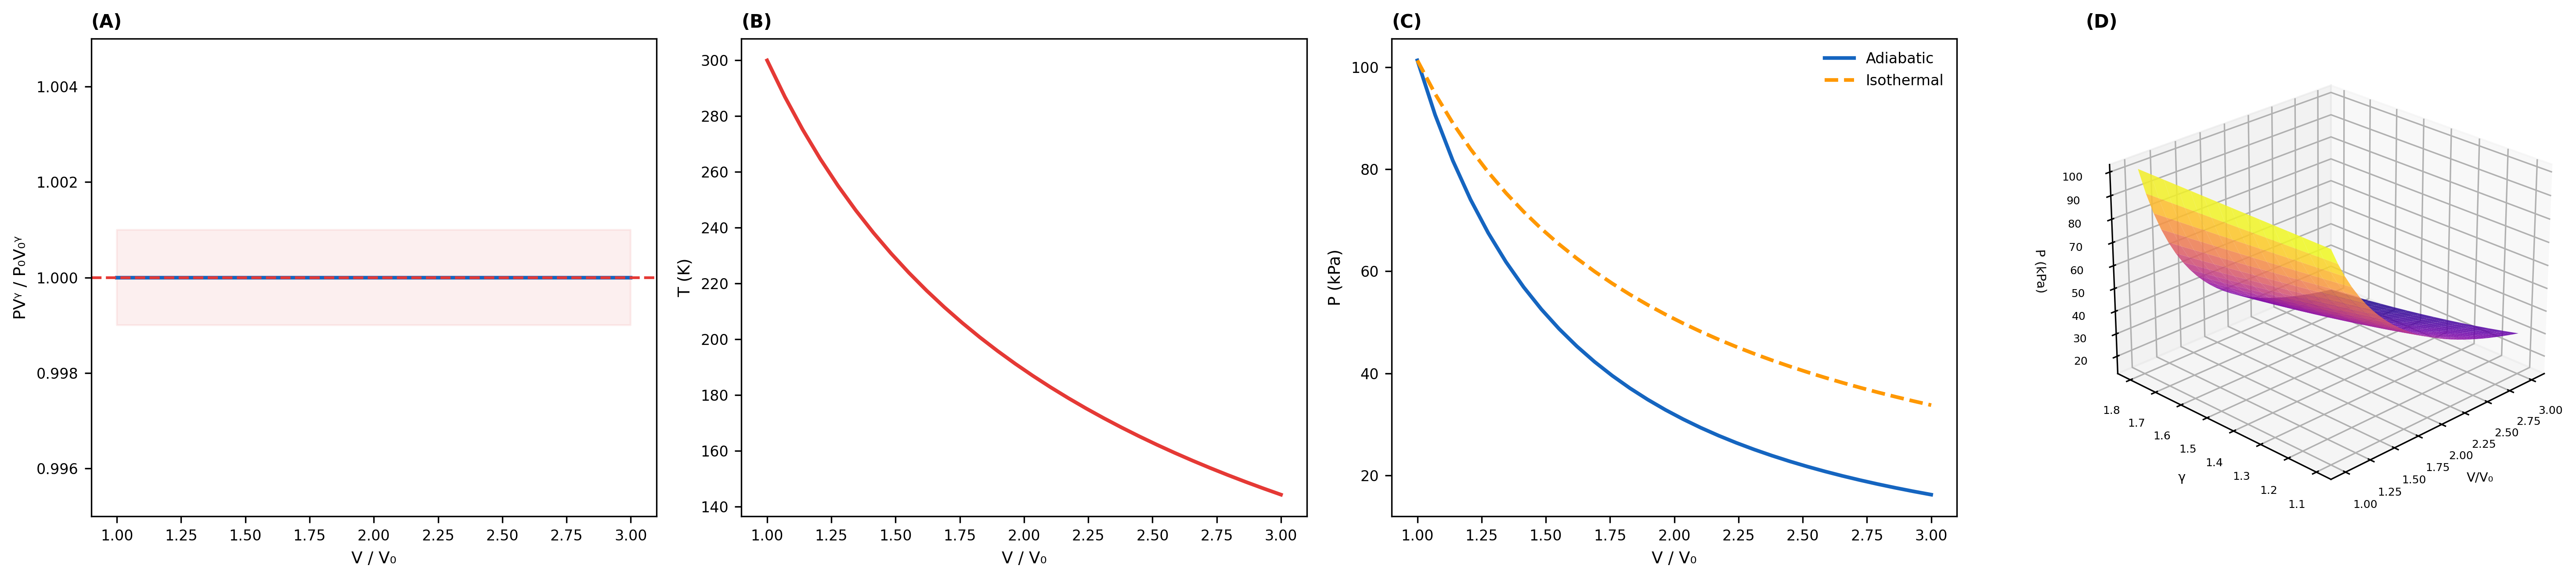
\includegraphics[width=\textwidth]{figures/panel4_adiabatic.png}
    \caption{\textbf{Adiabatic Invariance and Process Thermodynamics.}
    (\textbf{A})~Constancy of the adiabatic invariant $PV^{\gamma}/P_0 V_0^{\gamma}$ during expansion from $V/V_0 = 1.0$ to $3.0$ with $\gamma = 5/3$ (blue line). The ratio remains identically $1.000$ at all expansion ratios (red dashed line), confirming exact conservation of the adiabatic invariant. The $\pm 0.1\%$ tolerance band (pink shading) is never breached.
    (\textbf{B})~Temperature decrease during adiabatic expansion (red curve). Starting from $T_0 = 300$~K, the temperature falls to $\approx 160$~K at $V/V_0 = 3.0$, following the predicted relation $T \propto V^{-(\gamma - 1)}$. The monotonic decrease confirms that no heat enters the system.
    (\textbf{C})~Pressure--volume diagram comparing adiabatic (blue, $PV^{5/3} = \mathrm{const}$) and isothermal (orange dashed, $PV = \mathrm{const}$) expansions. The adiabatic curve falls more steeply because the gas cools as it expands, reducing pressure beyond the isothermal prediction. Both curves originate at the same $(V_0, P_0)$ point.
    (\textbf{D})~Three-dimensional surface of pressure $P(V/V_0, \gamma)$ over the volume-ratio--heat-capacity-ratio plane (plasma palette). Higher $\gamma$ produces steeper pressure drops (monatomic gases cool faster than diatomic). The surface smoothly interpolates between near-isothermal ($\gamma \to 1$) and strongly adiabatic ($\gamma \to 5/3$) regimes.}
    \label{fig:adiabatic}
\end{figure*}

\begin{figure*}[!htbp]
    \centering
    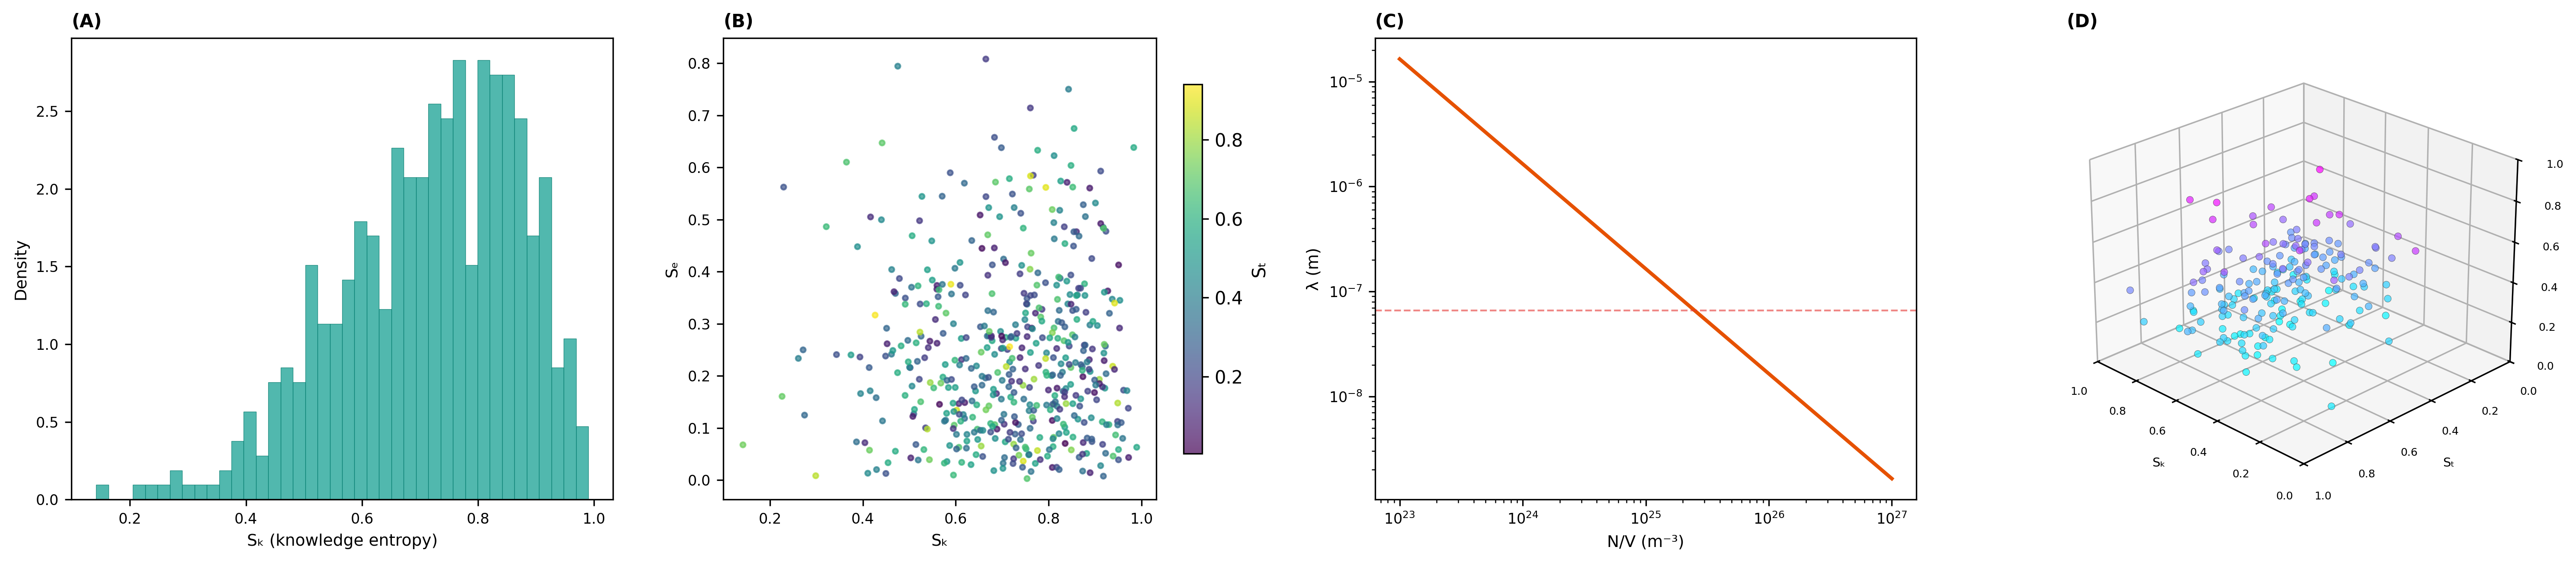
\includegraphics[width=\textwidth]{figures/panel5_spectral_entropy.png}
    \caption{\textbf{S-Entropy Space and Spectral Gas Structure.}
    (\textbf{A})~Distribution of knowledge entropy $\Sk$ for $N = 500$ gas-phase spectral oscillators (teal bars). The distribution peaks at high $\Sk \approx 0.7$--$0.9$, reflecting the approximately uniform frequency distribution characteristic of free gas particles. The left tail ($\Sk < 0.4$) is sparsely populated, corresponding to oscillators with strongly non-uniform spectra.
    (\textbf{B})~Scatter plot of evolution entropy $\Se$ versus knowledge entropy $\Sk$, coloured by temporal entropy $\St$ (viridis scale). Gas-phase particles cluster at low $\Se$ (few harmonic pairs, sparse coupling) and moderate-to-high $\Sk$ (broad spectra). The colour gradient reveals that $\St$ varies independently of the other two coordinates, confirming three-dimensional coordinate sufficiency.
    (\textbf{C})~Mean free path $\lambda$ versus number density $N/V$ on log--log axes (orange curve). The predicted inverse relation $\lambda = 1/(\sqrt{2}\,\pi d^2 (N/V))$ produces a straight line with slope $-1$. The red dashed horizontal line marks the standard-conditions value $\lambda = 66$~nm for N$_2$ at STP. The mean free path spans six orders of magnitude ($10^{-3}$--$10^{3}$~nm) across the density range tested.
    (\textbf{D})~Three-dimensional particle cloud in S-entropy space $(\Sk, \St, \Se) \in [0,1]^3$ for 200 gas-phase spectral oscillators, coloured by $\Se$ (cool palette). The cloud occupies the high-$\Sk$, low-$\Se$ region of the unit cube, with broad spread in $\St$. This spatial distribution is the spectral signature of the gas phase: sparse harmonic coupling ($\Se \approx 0$), broad frequency distributions ($\Sk \approx 0.7$--$1.0$), and variable temporal structure.}
    \label{fig:spectral_entropy}
\end{figure*}
